\section*{Solutions}


\begin{figure}[H]
\centering
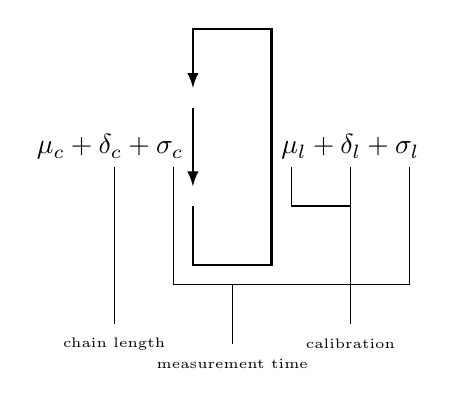
\begin{tikzpicture}

\draw [>=latex,->, line width = 0.3mm]
(0,1.25) |-
(1,0.5) --
(1,3.5) -|
(0,2.75);

\draw [>=latex,->, line width = 0.3mm]
(0,2.5) --
(0,1.5);

\node [anchor=west] at (1,2) {$\mu_l+\delta_{l}+\sigma_{l}$};
\node [anchor=east] at (0,2) {$\mu_c+\delta_{c}+\sigma_{c}$};

% measurement time
\draw (-0.25,1.75) -- (-0.25,0.25) -|  (0.5,-0.5);
\draw (0.5,0.25) -| (2.75,1.75);
\node at (0.5,-0.75) {\tiny{measurement time}};

% callibration
\draw (2,-0.25) -- (2,1.75);
\draw (1.25,1.75) |- (2,1.25);
\node at (2,-0.5) {\tiny{calibration}};

% chain length
\draw (-1,-0.25) -- (-1,1.75);

\node at (-1,-0.5) {\tiny{chain length}};
\end{tikzpicture}
\caption{math}
\label{tkz:math}
\end{figure}


\begin{align*}
\sigma_{tot} = \sqrt{\frac{\sigma_{c,s}^2}{\text{components}}+\frac{\sigma_{c,d}^2+\sigma_{l,d}^2}{\text{counts}}}
\end{align*}

\begin{align*}
LSB &= \frac{T}{\text{counts}\cdot \text{components}}\\
t_{meas} &= T\cdot \text{counts} = \frac{T^2}{LSB\cdot\text{components}}\\
\end{align*}

\begin{table}[H]
\centering
\caption{Requirements for $1\,ps$ resolution}
\label{my-label}
\begin{tabular}{|l|ll|ll|ll|ll|} \hline
ring size                     & 1         & 1         & 8         & 8         & 64          & 64          & 512           & 512        \\
component delay               & $50\,ps$  & $100\,ps$ & $50\,ps$  & $100\,ps$ & $50\,ps$    & $100\,ps$   & $50\,ps$      & $100\,ps$  \\ \hline
Period (T)                    & $50\,ps$  & $100\,ps$ & $400\,ps$ & $800\,ps$ & $3.2\,ns$   & $6.4\,ns$   & $25.6\,ns$    & $51.2\,ns$ \\
max counts                    & 50        & 100       & 50        & 100       & 50          & 100         & 50            & 100      \\
measurement time ($t_{meas}$) & $2.5\,ns$ & $10\,ns$  & $20\,ns$  & $80\,ns$  & $160\,ns$   & $640\,ns$   & $1.28\,\mu s$ & $5.12\,\mu s$  \\ \hline
\end{tabular}
\end{table}

for $N$ the number of elements in the Ring Oscillator
\begin{align*}
\Delta t_c &= \mathcal{N}(\mu_c,\sigma_c^2)\\
\Delta t_{RO}&= \mathcal{N}(N\mu_c,\sqrt{N}\sigma_{c}^2)\\
\frac{\Delta t_{RO}}{N}&= \mathcal{N}(\mu_c,\frac{\sigma_{c}^2}{\sqrt{N}}) 
\end{align*}
for $N$ the number of elements in the Ring Oscillator\\
for $C$ the number of counts
\begin{align*}
t_c &= \mathcal{N}(\Delta t_c,\sigma_d^2)\\
t_{RO}&= \mathcal{N}(C\Delta t_{RO},\sqrt{NC}\sigma_{d}^2) \\
\frac{t_{RO}}{NC}&= \mathcal{N}(\frac{\Delta t_{RO}}{N},\frac{\sigma_{d}^2}{\sqrt{NC}}) 
\end{align*}